
In dem Teil wird die komplete innere Logik der Application beschrieben. Dafür ist nur \textbf{Controller} notwendig. 
D.h. beim Geschehen eines Ereignisses wird eine (oder mehrere) Method(en) in deb jeweiligen Controllern aufgerufen,
die das Ereignis entsprechend abarbeiten.
Dabei entsteht das Problem, dass
jeder \textbf{Controller} mehrere Aufgaben übernimmt 
(z.B. Kontrollieren von \textbf{Port} und \textbf{Adapter} und enthält Anwendungslogik).
Das wiederspricht dem \textbf{SRP}, das in dem Kapitel \ref{kap:SRP} beschrieben ist.

Eine mögliche Lösung wäre das Separieren von Kontrollieren von \textbf{Port} und \textbf{Adapter} und Anwendungslogik
in zwei verschiedenen Teile. Die Anwendungslogik heißt \textbf{UseCase}.

Bei dieser Aufteilung besteht das Problem, dass beim Auftreten eines Ereignisses im \textbf{Controller} muss dieses Ereignis an das 
richtige \textbf{UseCase} zugeordnet werden. D.h. \textbf{Contoller} besitzt eine weitere Verantwortlichkeit die sich in ein anderes Teil
verschieben lässt. Dieses Teil heißt \textbf{Dispatcher} und seine Aufgabe ist alle Abonnenten \textbf{UseCase}s
beim Auftreten eines Ereignisses zu informieren.

Jedes \textbf{UseCase} kann mehrere aufeinander folgende Aufgaben erledigen.
Alle Aufgaben müssen gleiche Funktionalitäten besitzen, z.B:
\begin{itemize}
    \item der Anfang und das Ende in Logs aufzeichnen.
    \item Nach einer bestimmten Zeit gestoppt werden.
\end{itemize}
D.h. man braucht eine ``Hülle'' um jeder Methode - \textbf{Interactor}

Wenn alles zusammengeführt wird, entsteht folgendes Objektendiamm:

\begin{figure}[H]
    \centering
    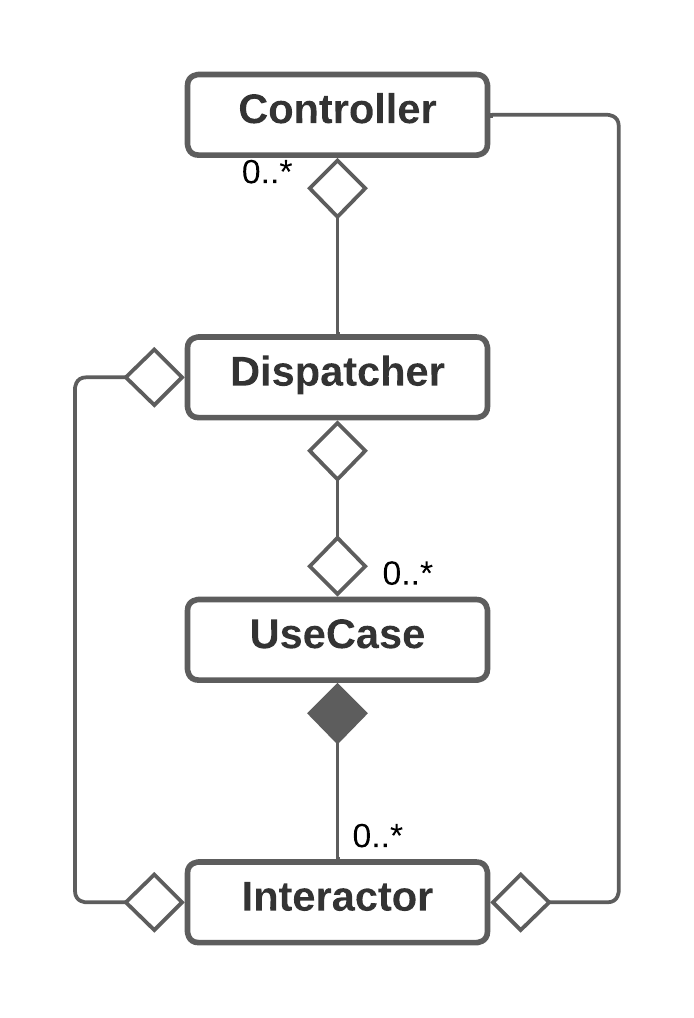
\includegraphics[width=6.5cm]{./images/Controller-Dispatcher-UseCase-Interactor.png}
     \caption[Objektendiagramm Controller-Dispatcher-UseCase-Interactor]{Objektendiagramm Controller-Dispatcher-UseCase-Interactor}
     \label{fig:CDCDUI}
\end{figure}
